\section{Приложение} \label{Приложение}

\subsection{Приложение 1} \label{Приложение 1}
Схема экспериментальной установки приведена на рис. 1
\begin{figure}[ht]
    \center{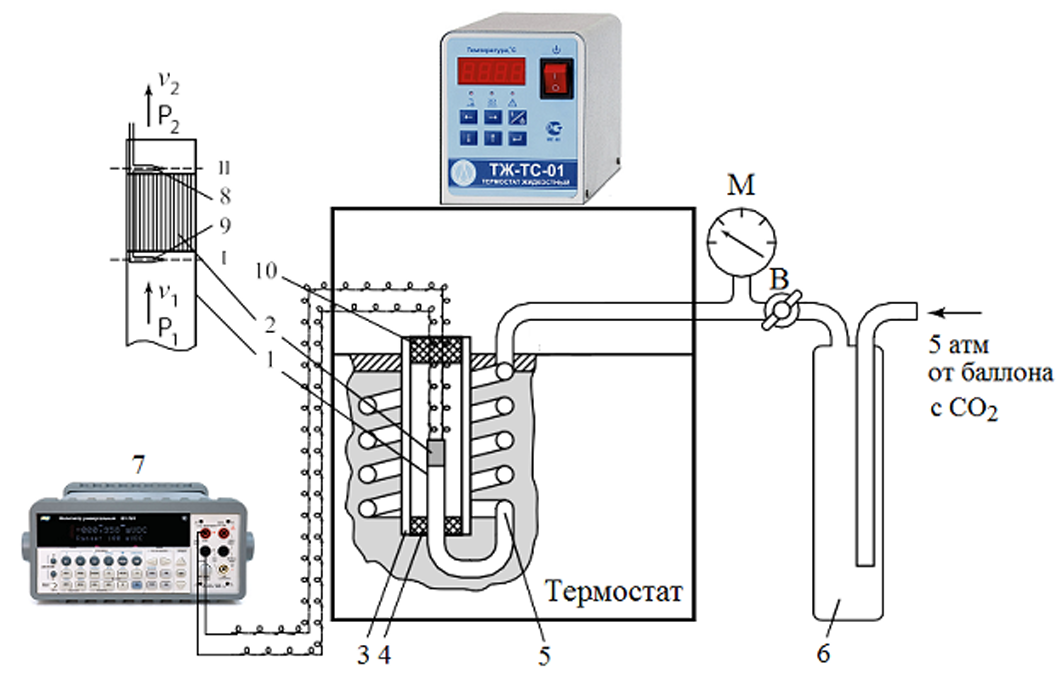
\includegraphics[scale=0.5]{img/exp_ustanovka_3.png}}
    \begin{center}       
        Рис. 1. Экспериментальная установка для измерения зависимости $\Delta T(\Delta P)$
    \end{center}
\end{figure}

Установка состоит из трубки 1 с пористой перегородкой 2, через которую пропускается углекислый газ. Трубка сделана из нержавеющей стали, обладающей малой теплопроводностью. Пористая перегородка представляет собой стеклянную пористую пробку со множеством узких и длинных каналов. Углекислый газ поступает в трубку через змеевик 5 из балластного баллона 6. Медный змеевик омывается водой термостата и нагревает протекающий через него газ до температуры, установленной на термостате. В трубу напуска газа встроен манометр М и вентиль В для регулировки давления газа. К торцам перегородки подключены спаи 8 и 9 дифференциальной термопары медь-константан. Константановая проволока соединяет спаи, а медные проволоки подсоединены к цифровому вольтметру 7. Трубка с пористой перегородкой помещена в трубу Дьюара 3, стенки которой посеребрены, для уменьшения теплоотдачи, связанной с излучением. Для уменьшения теплопотерь за счет конвекции труба Дьюара закрыта с торцов кольцом 4 и пробкой 10 из пенопласта.

\subsection{Приложение 2} \label{Приложение 2}
Для определения разности $\Delta T$ температур газа на входе и выходе из трубки используется дифференциальная термопара константан-медь, подключенная к цифровому мультиметру. Напряжение $U$ на мультиметре пропорционально разности $\Delta T$ температур спаев термопары
\begin{equation}
    U = \beta\Delta T \label{eq: E}
\end{equation}

$\beta$ - чувствительность термопары, которая зависит от диапазона температур, в котором производится измерение. Значения $\beta$ при различных диапазонах температур приведены в таблице 1.

\begin{table}[h]
    \centering
    \begin{tabular}{|c|c|c|c|c|c|}
    \hline
    $T, \celsius$                        & 0-10 & 10-20  & 20-30  & 30-40  & 40-50 \\ \hline
    $\beta, \frac{\text{мкВ}}{\celsius}$ & 38.9 & 39.8   & 40.7   & 41.6   & 42.5 \\ \hline
    $T, \celsius$                        & 50-60 & 60-70  & 70-80  & 80-90  & 90-100 \\ \hline
    $\beta, \frac{\text{мкВ}}{\celsius}$ & 43.3  & 44.1   & 44.9   & 45.6   & 46.4 \\ \hline
\end{tabular}
    \caption{Чувствительность $\beta$ термопары в различных диапазонах температур $T$}
    \label{tab:t1}
\end{table}

\subsection{Приложение 3} \label{Приложение 3}
\begin{table}[h]
    \centering
    \begin{tabular}{|c|c|c|c|c|c|}
    \hline
    $\Delta P, \text{атм}$ & $U, \text{мВ}$ & $\Delta T, \celsius$  & $\sigma_{\Delta T}, \celsius$  & $\sigma_{\Delta P}, \text{атм}$ & $\sigma_U\cdot 10^{-3}, \text{мВ}$ \\ \hline
     -4.0 & -0.163  & -4.1   & 0.05   & 0.1   & 2 \\ \hline
     -3.5 & -0.136  & -3.4   & 0.05   & 0.1   & 2 \\ \hline
     -3.0 & -0.117  & -2.9   & 0.05   & 0.1   & 2 \\ \hline
     -2.5 & -0.093  & -2.3   & 0.05   & 0.1   & 2 \\ \hline
     -2.0 & -0.069  & -1.9   & 0.05   & 0.1   & 2 \\ \hline
     -1.5 & -0.047  & -1.5   & 0.05   & 0.1   & 2 \\ \hline
\end{tabular}
    \caption{Зависимость разности $\Delta P$ давлений газа на выходе из трубки и на входе в нее от разности $\Delta T$ температур по разные стороны от перегородки при температуре $T = 18\celsius$ , $U$ - показания мультиметра, $\sigma_{\Delta T}, \sigma_{\Delta P}, \sigma_U$ - погрешности измерения $\Delta T, \Delta P, U$ соответственно}
    \label{tab:t1}
\end{table}

\begin{table}[h]
    \centering
    \begin{tabular}{|c|c|c|c|c|c|}
    \hline
    $\Delta P, \text{атм}$ & $U, \text{мВ}$ & $\Delta T, \celsius$  & $\sigma_{\Delta T}, \celsius$  & $\sigma_{\Delta P}, \text{атм}$ & $\sigma_U\cdot 10^{-3}, \text{мВ}$ \\ \hline
     -4.0  & -0.147  & -3.6   & 0.05   & 0.1   & 2 \\ \hline
     -3.5  & -0.123  & -3.0   & 0.05   & 0.1   & 2 \\ \hline
     -3.1  & -0.102  & -2.5   & 0.05   & 0.1   & 2 \\ \hline
     -2.5  & -0.080  & -2.0   & 0.05   & 0.1   & 2 \\ \hline
     -2.0  & -0.060  & -1.5   & 0.05   & 0.1   & 2 \\ \hline
     -1.55 & -0.040  & -1.0   & 0.05   & 0.1   & 2 \\ \hline
\end{tabular}
    \caption{Зависимость разности $\Delta P$ давлений газа на выходе из трубки и на входе в нее от разности $\Delta T$ температур по разные стороны от перегородки при температуре $T = 30\celsius$ , $U$ - показания мультиметра, $\sigma_{\Delta T}, \sigma_{\Delta P}, \sigma_U$ - погрешности измерения $\Delta T, \Delta P, U$ соответственно}
    \label{tab:t1}
\end{table}

\begin{table}[h]
    \centering
    \begin{tabular}{|c|c|c|c|c|c|}
    \hline
    $\Delta P, \text{атм}$ & $U, \text{мВ}$ & $\Delta T, \celsius$  & $\sigma_{\Delta T}, \celsius$  & $\sigma_{\Delta P}, \text{атм}$ & $\sigma_U\cdot 10^{-3}, \text{мВ}$ \\ \hline
     -4.0  & -0.130  & -3.1   & 0.05   & 0.1   & 2 \\ \hline
     -3.5  & -0.105  & -2.5   & 0.05   & 0.1   & 2 \\ \hline
     -2.9  & -0.080  & -1.9   & 0.05   & 0.1   & 2 \\ \hline
     -2.6  & -0.066  & -1.6   & 0.05   & 0.1   & 2 \\ \hline
     -2.0  & -0.042  & -1.0   & 0.05   & 0.1   & 2 \\ \hline
     -1.5  & -0.028  & -0.7   & 0.05   & 0.1   & 2 \\ \hline
\end{tabular}
    \caption{Зависимость разности $\Delta P$ давлений газа на выходе из трубки и на входе в нее от разности $\Delta T$ температур по разные стороны от перегородки при температуре $T = 40\celsius$ , $U$ - показания мультиметра, $\sigma_{\Delta T}, \sigma_{\Delta P}, \sigma_U$ - погрешности измерения $\Delta T, \Delta P, U$ соответственно}
    \label{tab:t1}
\end{table}

\begin{table}[h]
    \centering
    \begin{tabular}{|c|c|c|c|c|c|}
    \hline
    $\Delta P, \text{атм}$ & $U, \text{мВ}$ & $\Delta T, \celsius$  & $\sigma_{\Delta T}, \celsius$  & $\sigma_{\Delta P}, \text{атм}$ & $\sigma_U\cdot 10^{-3}, \text{мВ}$ \\ \hline
     -4.0  & -0.103  & -2.4   & 0.05   & 0.1   & 2 \\ \hline
     -3.4  & -0.079  & -1.9   & 0.05   & 0.1   & 2 \\ \hline
     -3.0  & -0.062  & -1.5   & 0.05   & 0.1   & 2 \\ \hline
     -2.5  & -0.046  & -1.1   & 0.05   & 0.1   & 2 \\ \hline
     -2.0  & -0.031  & -0.7   & 0.05   & 0.1   & 2 \\ \hline
     -1.5  & -0.021  & -0.3   & 0.05   & 0.1   & 2 \\ \hline
\end{tabular}
    \caption{Зависимость разности $\Delta P$ давлений газа на выходе из трубки и на входе в нее от разности $\Delta T$ температур по разные стороны от перегородки при температуре $T = 50\celsius$ , $U$ - показания мультиметра, $\sigma_{\Delta T}, \sigma_{\Delta P}, \sigma_U$ - погрешности измерения $\Delta T, \Delta P, U$ соответственно}
    \label{tab:t1}
\end{table}
\newpage
\subsection{Приложение 4} \label{Приложение 4}
\begin{table}[h]
    \centering
    \begin{tabular}{|c|c|c|c|c|}
    \hline
    $T, \celsius$ & $T^{-1}\cdot 10^{-3}, K^{-1}$ & $\mu_{\text{д-т}}\cdot 10^{-5}, \frac{K}{\text{Па}}$  & $\sigma_{\mu_{\text{д-т}}}\cdot 10^{-5}, \frac{K}{\text{Па}}$ & $\sigma_{T^{-1}}\cdot 10^{-6}, K^{-1}$ \\ \hline
     18  & 3.4  & 1.03   & 0.05 & 1.18  \\ \hline
     30  & 3.3  & 0.98   & 0.03 & 1.09  \\ \hline
     40  & 3.2  & 0.92   & 0.04 & 1.02 \\ \hline
     50  & 3.1  & 0.84   & 0.01 & 0.96 \\ \hline
\end{tabular}
    \caption{Зависимость температуры $T$ газа на входе в трубку от коэффициента $\mu_\text{д-т}$ Джоуля-Томсона, $\sigma_{\mu_{\text{д-т}}}$ - погрешность вычисления $\mu_\text{д-т}$, $\sigma_{T^{-1}}$ - погрешность вычисления $T^{-1}$}
    \label{tab:t1}
\end{table}
\newpage
\subsection{Приложение 5} \label{Приложение 5}
\begin{table}[h]
    \centering
    \begin{tabular}{|c|c|c|c|}
    \hline
    $k \cdot 10^{-3}, \frac{K^2}{\text{Па}}$ & 
    $t\cdot 10^{-3}, \frac{K}{\text{Па}}$ &
    $a, \frac{\text{Па}\cdot \text{м}^6}{\text{моль}^2\cdot K}$  &
    $b\cdot 10^{-3}, \frac{\text{м}^3}{\text{моль}}$ \\ \hline
     6.3  & -1.11  & 0.76   & 0.32 \\ \hline
    $\sigma_k\cdot 10^{-3}, \frac{K^2}{\text{Па}}$ &
    $\sigma_t\cdot 10^{-6}, \frac{K}{\text{Па}}$ &
    $\sigma_a, \frac{\text{Па}\cdot \text{м}^6}{\text{моль}^2\cdot K}$ & $\sigma_b\cdot 10^{-5}, \frac{\text{м}^3}{\text{моль}}$\\ \hline
     0.48 & 1.56 & 0.06 & 4.55  \\ \hline
\end{tabular}
    \caption{Значения коэффициентов $a, b$ уравнения Ван-дер-Ваальса для углекислого газа. $k$ - угловой коэффициент графика зависимости $\mu_\text{д-т}(T^{-1})$, $t$ - свободный член графика зависимости $\mu_\text{д-т}(T^{-1})$, $\sigma_k, \sigma_t, \sigma_a, \sigma_b$ - погрешности вычисления $k, t, a, b$ соответственно.}
    \label{tab:t1}
\end{table}
\subsubsection{Формулы для вычисления коэффициентов $a, b$ из выражения \eqref{eq: mu}}

\begin{equation}
    a = \frac{R c_p k}{2}
\end{equation}
\begin{equation}
    b = -t\cdot c_p
\end{equation}
$R = 8.31\frac{\text{Дж}}{\text{моль}\cdot K}$ - универсальная газовая постоянная, $c_p = 29.14 \frac{\text{Дж}}{\text{моль}\cdot K}$ - молярная теплоемкость углекислого газа при постоянном давлении, $k$ - угловой коэффициент графика $\mu_\text{д-т}(T^{-1})$, $t$ - свободный член графика зависимости $\mu_\text{д-т}(T^{-1})$.

\subsection{Приложение 6} \label{Приложение 6}
\begin{table}[h]
    \centering
    \begin{tabular}{|c|c|c|c|}
    \hline
    $\text{Вещество}$ & 
    $a, \frac{\text{Па}\cdot \text{м}^6}{\text{моль}^2\cdot K}$  &
    $b\cdot 10^{-5}, \frac{\text{м}^3}{\text{моль}}$ &
    $T_\text{инв}, K$ \\ \hline
     водяной пар  & 0.556  & 3.06 & 4370 \\ \hline
     углекислый газ & 0.364 & 4.26 & 1500 \\ \hline
     кислород & 0.136 & 3.16 & 771 \\ \hline
     аргон & 0.136 & 3.22 & 760\\ \hline
     азот & 0.136 & 3.85 & 604 \\ \hline
     водород & 0.0244 & 2.63 & 264 \\ \hline
     гелий & 0.00343 & 2.34 & 40 \\ \hline
\end{tabular}
    \caption{Коэффициенты $a, b$ в уравнении Ван-дер-Ваальса и температура $T_\text{инв}$ инверсии для различных веществ.}
    \label{tab:t1}
\end{table}

\subsection{Формулы для расчета погрешностей} \label{Приложение 7}
\subsubsection{Расчет погрешности углового коэффициента графика $\Delta T(\Delta P)$}
\[\sigma_{\mu_\text{д-т}} = \frac{1}{\sqrt{n}}\sqrt{\frac{\langle \Delta T^2 \rangle - {\langle \Delta T \rangle}^2}{\langle \Delta P^2 \rangle - {\langle \Delta P \rangle}^2} - \mu_\text{д-т}^2}\] $n$ - количество экспериментальных точек.
\subsubsection{Расчет погрешности углового коэффициента и свободного члена графика $\mu_\text{д-т}(T^{-1})$}
\[\sigma_{k} = \frac{1}{\sqrt{n}}\sqrt{\frac{\langle \mu_\text{д-т}^2 \rangle - {\langle \mu_\text{д-т} \rangle}^2}{\langle (T^{-1})^2 \rangle - {\langle T^{-1} \rangle}^2} - k^2}\]
\[\sigma_t = \sigma_{k} \cdot \sqrt{\langle (T^{-1})^2 \rangle - {\langle T^{-1} \rangle}^2}\]
\subsubsection{Расчет погрешности коэффициентов $a, b$}
\[\sigma_a = \frac{Rc_p}{2}\cdot \sigma_K\]
\[\sigma_b = c_p \cdot \sigma_t\]
\subsubsection{Расчет погрешности $T_\text{инв}$}
\[ \sigma_{T_{инв}} = \sqrt{(\frac{2}{Rb})^2\cdot \sigma_a^2 + (\frac{2a}{Rb^2})^2\cdot \sigma_b^2} = \frac{2}{Rb^2}\sqrt{\sigma_a^2\cdot b^2 + \sigma_b^2\cdot a^2}\]
\subsubsection{Расчет погрешности $\Delta T$}
\[\sigma_{\Delta T} = \frac{\sigma_U}{\beta}\]